\documentclass[conference]{IEEEtran}
\IEEEoverridecommandlockouts
% The preceding line is only needed to identify funding in the first footnote. If that is unneeded, please comment it out.
\usepackage{cite}
\usepackage{amsmath,amssymb,amsfonts}
\usepackage{algorithmic}
\usepackage{graphicx}
\usepackage{textcomp}
\usepackage{xcolor}
\usepackage{blindtext}
\usepackage{hyperref}
\usepackage[spanish]{babel}
\def\BibTeX{{\rm B\kern-.05em{\sc i\kern-.025em b}\kern-.08em
    T\kern-.1667em\lower.7ex\hbox{E}\kern-.125emX}}
\begin{document}

\title{Implementación de enlaces punto a punto
}

\author{\IEEEauthorblockN{Germán Eduardo Castro Burgos}
\IEEEauthorblockA{\textit{Ingeniería de RF} \\
\textit{Universidad de Nariño}\\
Pasto, Colombia \\
$german\_castrob@hotmail.com$}
}
\maketitle

\section{Introducción}
La creciente necesidad de acceso a recursos informáticos ha traído consigo durante las últimas décadas,
un incipiente auge en el desarrollo de tecnologías que faciliten la implementación de sistemas de comunicaciones
en diversos escenarios rurales y urbanos. Las barreras topográficas existentes en algunas regiones, han determinado
en ocasiones la imposibilidad de brindar una solución factible para garantizar la conectividad de la región considerada, 
generando efectos adversos sobre la economía, educación y en general la calidad de vida de quienes habitan estas zonas.
Para mitigar los efectos descritos, diferentes alternativas tecnológicas se han propuesto considerando diversas metodologías
y medios de transmisión. Inicialmente los sistemas de comunicaciones basados en un medio físico (cable) contaban con capacidades
operativas significativamente superiores cuando su desempeño se contrastaba con el de sistema inalámbricos, que se veían limitados
por la cantidad de información que podía ser transferida luego de su despliegue. 

Con el incremento en la capacidad de procesamiento de sistemas embebidos y el surgimiento de nuevas técnicas de modulación de 
señales, la brecha entre sistemas inalámbricos y cableados se ha visto disminuida. Como resultado, la implementación de sistemas 
inalámbricos en áreas rurales o de dificil acceso es cada día mas frecuente. Los radioenlaces se presentan en dicho panorama, 
como una solución costo-efectiva para garantizar el acceso de comunidades aisladas a servicios de internet, y para establecer redes de 
comunicaciones multi propósito que contribuyen a garantizar la seguridad de la comunidad. El éxito de la solución propuesta estará 
relacionado con las consideraciones efectuadas durante la fase de diseño del enlace a emplear, siendo fundamentales la selección de los 
dispositivos que harán parte del sistema y la caracterización del enlace inalámbrico a partir de cálculos teóricos que requieren del uso 
de modelos de propagación y del reconocimiento de las regiones de Fresnel asociadas al escenario de trabajo. Este documento resume el procedimiento
llevado a cabo para la implementación de un enlace inalámbrico punto a punto, señalando las principales características de los elementos empleados,
las consideraciones previas a la implementación del enlace y un análisis comparativo de los resultados obtenidos frente a los pronósticos 
efectuados mediante la aplicación de las relaciones teóricas existentes para diferentes modelos de propagación.
\section{Descripción del experimento efectuado}
El ejercicio efectuado en busca de identificar las etapas que deben recorrerse para implementar de forma exitosa un radio enlace, tuvo como 
punto de partida la selección de los dispositivos a emplear para establecer la comunicación bi-direccional entre dos equipos terminales. Dado que el 
enlace propuesto corresponde en su configuración a un esquema punto a punto, en el que las comunicaciones se entablan exclusivamente entre dos
únicos nodos, es necesario implementar dos estaciones idénticas que permitan la transmisión de paquetes entre dos equipos de cómputo conectados
a cada extremo del enlace. Para identificar los efectos ocasionados sobre la potencia recibida en uno de los extremos del enlace, cuando se delimita
la primera zona de Fresnel, un obstáculo ha sido posicionado en el punto medio de la distancia que separa las estaciones transmisoras en busca de que
la señal reflejada sobre el mismo incremente el nivel de la potencia recibida. El escenario descrito puede apreciarse en la Figura @.
\begin{figure}
    \centering
          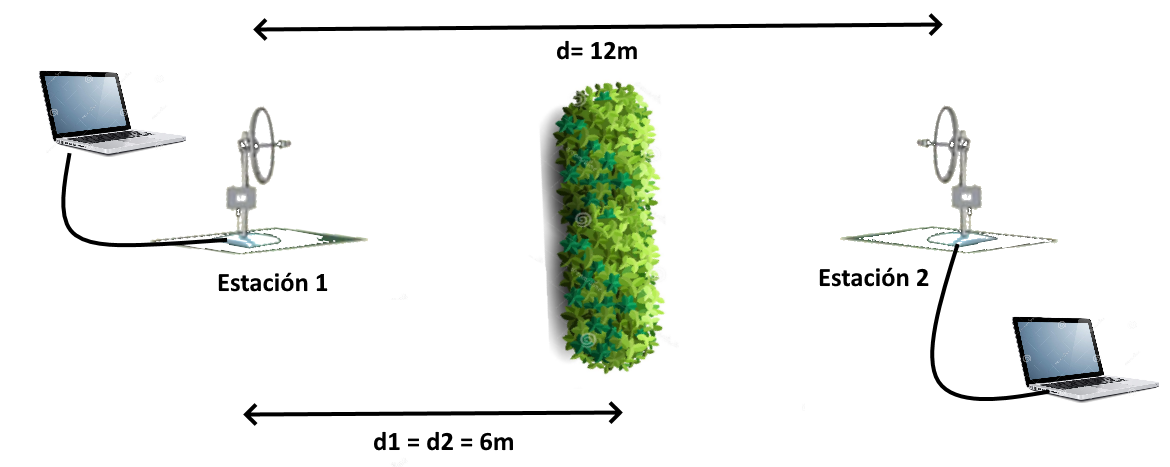
\includegraphics[width=0.47\textwidth]{Escenario.png}
        \caption{Antena tipo Rubber Duck HG2458-5RD-RSP.
        }
        \label{fig:Escenario}
\end{figure}
\subsection{Instrumentación empleada}
Cada una de las estaciones transmisoras está constituida por un conjunto antena-radio encargado de entablar comunicaciones con el nodo ubicado al 
otro extremo del enlace.
\end{document}